\section{Tool Evidence Controls the Agent Workflow}
\label{sec:vcl}

The task interface exposes an editable kernel, public tests, target part, and
budgets while withholding hidden tests and frozen references. The controller
records every candidate, gate, metric, token, and credit in one run state.

The \VCL{} runs seven gates in order: Interface, \CSim, \Synth, Frequency,
Capacity, required \CoSim, and Metric completeness. Frequency enforces
100\,MHz, Capacity enforces U55C limits, and \CoSim{} applies only when
required. Define validity $V(c)=\prod_i G_i$ over applicable gates
$G_i\in\{0,1\}$; an inapplicable gate contributes $1$. Let $b$ be the
verified fallback. The promotion rule is
$P(c)=V(c)\land[Q_{\mathrm{HW}}(c)>Q_{\mathrm{HW}}(b)]$.

Local failure classification and retrieval require no additional model call;
generating a subsequent candidate still does. \textbf{Failure Reflection}
parses interface, synthesis, and co-simulation diagnostics plus the source
diff into a compact constraint for the next proposal. \textbf{QoR-RAG}
retrieves compatible public rules and measured success/failure cases by task
metadata and bottleneck, then adds them to the optimization context. Thus
interface mismatches produce signature/pragma constraints, synthesis failures
produce timing/resource/II constraints, and co-simulation deadlocks produce
handshake/port-width constraints. Duplicate candidates and repeated failures
stop retries.

Figure~\ref{fig:vcl} summarises the loop. The controller records every
candidate and gate outcome for audit, while a failed or incomplete candidate
never replaces the last verified fallback.

\begin{figure*}[t]
  \centering
  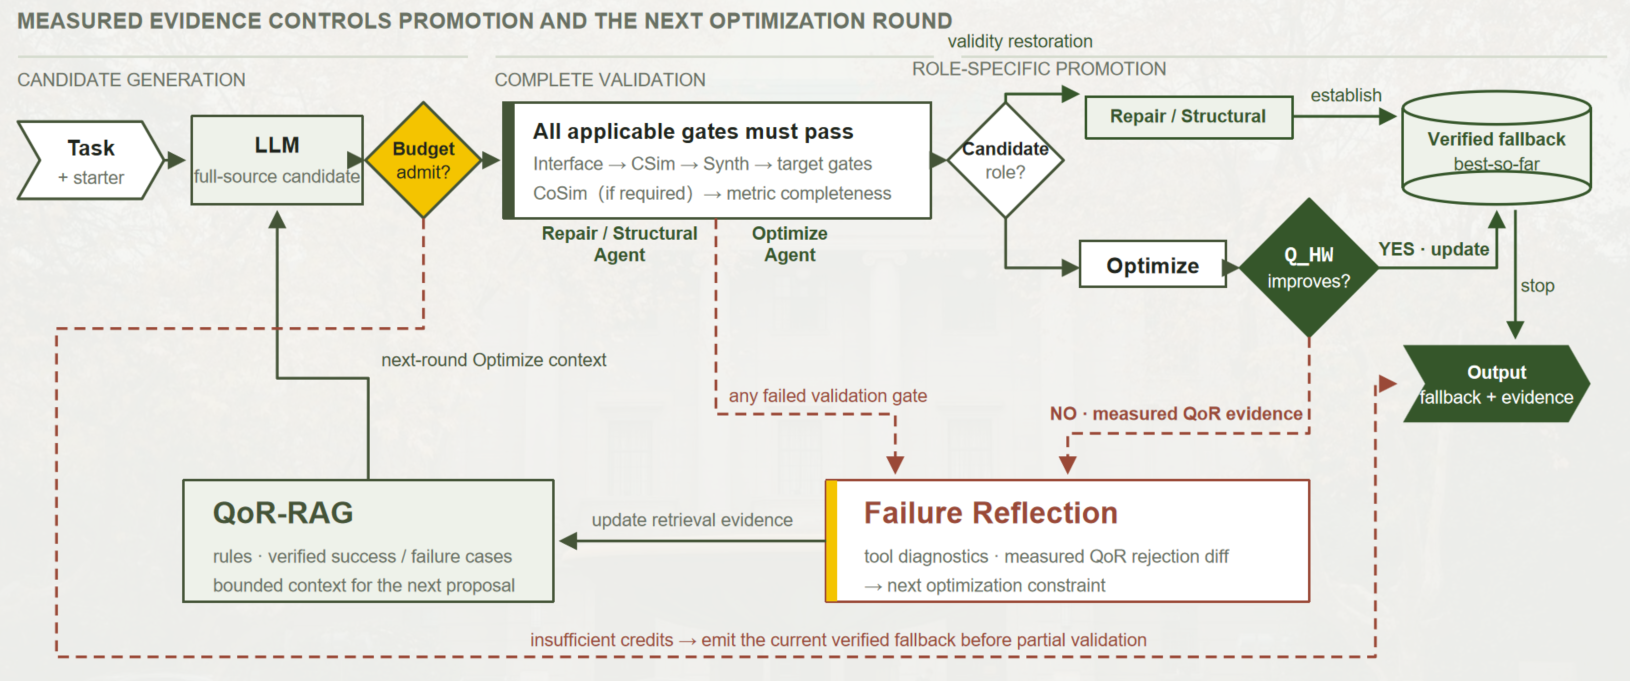
\includegraphics[width=0.84\textwidth]{系统框图.png}
  \vspace{-4pt}
  \caption{\textbf{The Verified-Candidate Loop.} A candidate replaces the
  verified fallback only after every applicable gate passes and the composite
  $Q_{\mathrm{HW}}$ improves.}
  \label{fig:vcl}
  \vspace{-6pt}
\end{figure*}
